\chapter{INSTALASI QGIS}

Cara instalasi aplikasi QGIS berbeda antara menggunakan sistem operasi Windows dan sistem operasi Linux.

\begin{enumerate}[A.]

\item Instalasi QGIS di lingkungan Sistem Operasi Windows

Untuk sistem operasi Windows, perangkat lunak QGIS dapat di unduh secara gratis di \textit{website} resmi QuantumGIS dengan alamat http://qgis.org/ melalui berbagai macam \textit{web browser} seperti Firefox, Chrome, Opera, atau Internet Explorer. Tahapannya adalah sebagai berikut :

\begin{enumerate}[1.]

\item Pada kolom halaman di atas jendela \textit{browser}, masukan teks berikut dan tekan Enter : http://qgis.org/, sehingga muncul jendela pada gambar \ref{fig:qgishomepage} :

\begin{figure}[H]
  \centering
  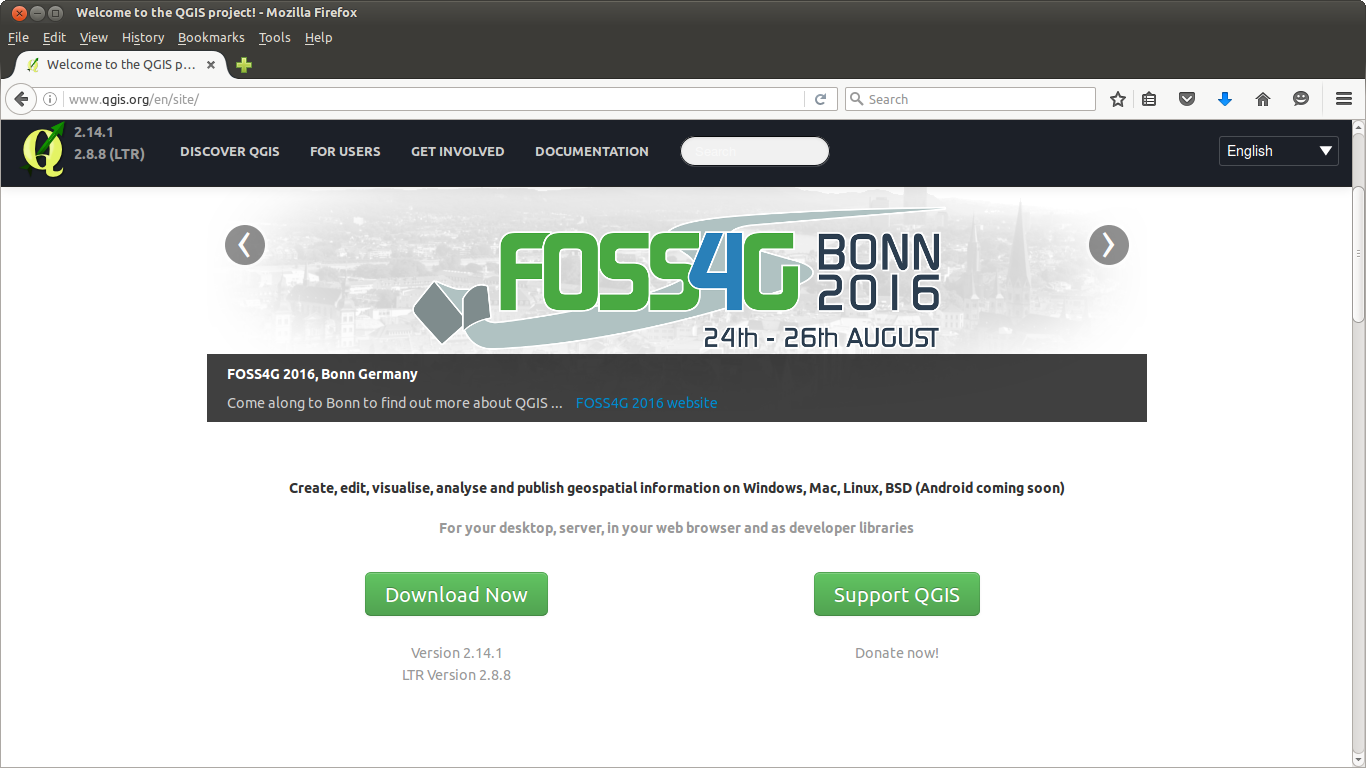
\includegraphics[width=1\textwidth]{./resources/001-homepage-qgis}
  \caption{Jendela \textit{website} QGIS}
  \label{fig:qgishomepage}
\end{figure}

\item Klik \verb|Download Now| pada halaman tersebut.

\item Pada jendela \textit{download} seperti ditampilkan dalam gambar \ref{fig:qgisversion} akan terdapat pilihan QGIS \textit{installer} berdasarkan sistem operasi perangkat yang anda gunakan. \textit{Expand} pilihan sistem operasi yang anda gunakan, lalu klik pada \textbf{Standalone Installer} (direkomendasikan untuk pengguna pemula).

\begin{figure}[H]
  \centering
  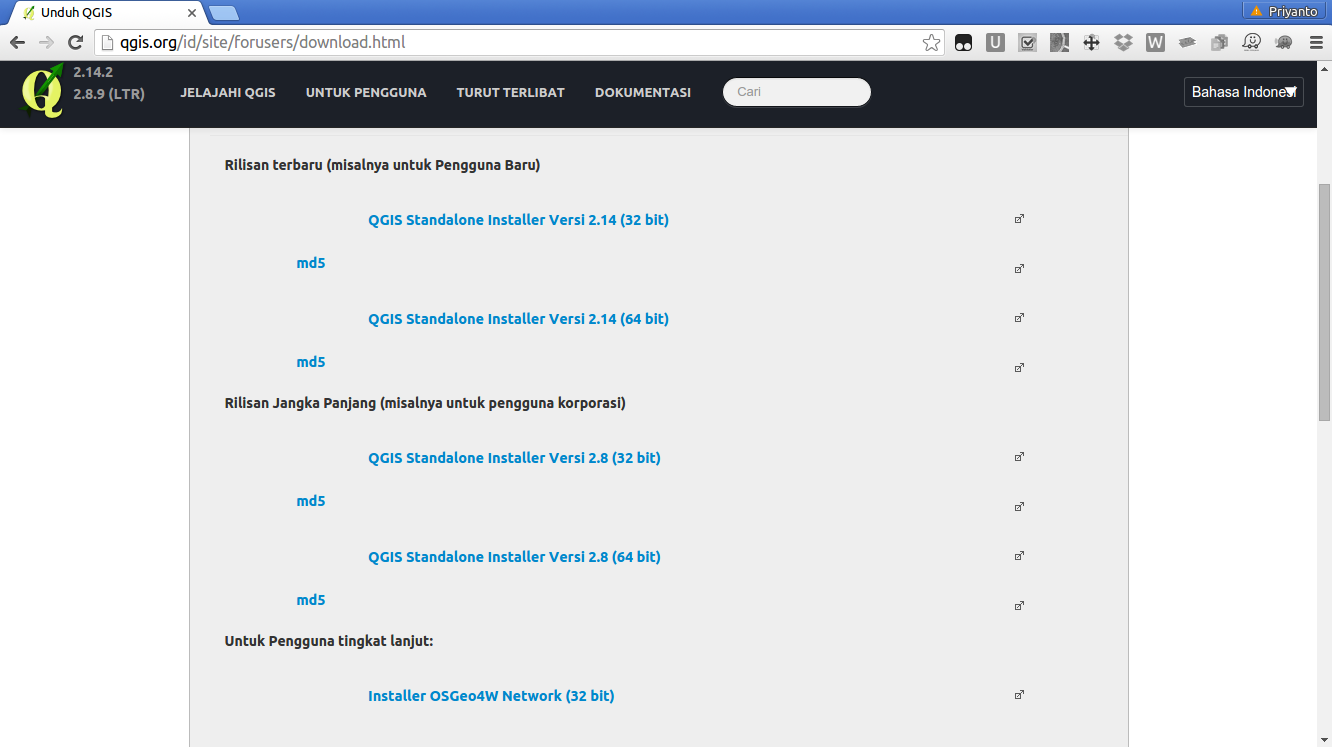
\includegraphics[width=1\textwidth]{./resources/002-pilihan-versi}
  \caption{Pilihan Versi QGIS}
  \label{fig:qgisversion}
\end{figure}

\item Apabila QGIS telah berhasil diunduh, cari \textit{file} instalasi pada direktori yang telah anda tentukan sebelumnya. Mungkin akan terlihat seperti gambar \ref{fig:qgisinstaller} :

\begin{figure}[H]
  \centering
  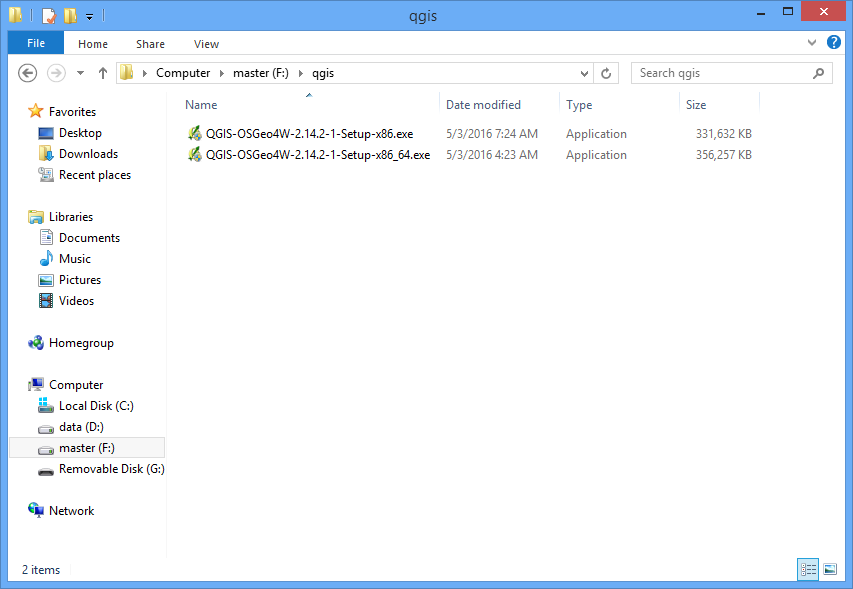
\includegraphics[width=0.9\textwidth]{./resources/install-win/001-file-installer-qgis}
  \caption{\textit{File installer} QGIS}  
  \label{fig:qgisinstaller}
\end{figure}

\item Klik dua kali pada \textit{file} instalasi tersebut untuk memulai penginstalan QGIS. Nantinya akan muncul tampilan seperti gambar \ref{fig:welcomeinstall}

\begin{figure}[H]
  \centering
  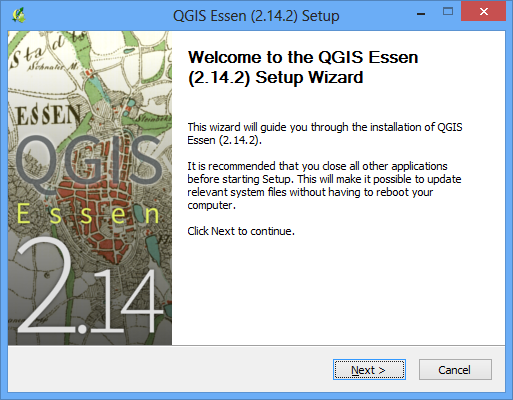
\includegraphics[width=0.9\textwidth]{./resources/install-win/002-welcome}
  \caption{Tampilan Awal Instalasi QGIS}
  \label{fig:welcomeinstall}
\end{figure}

\item Langsung saja tekan tombol \textit{Next} sehingga muncul tampilan seperti gambar \ref{fig:agreement}

\begin{figure}[H]
  \centering
  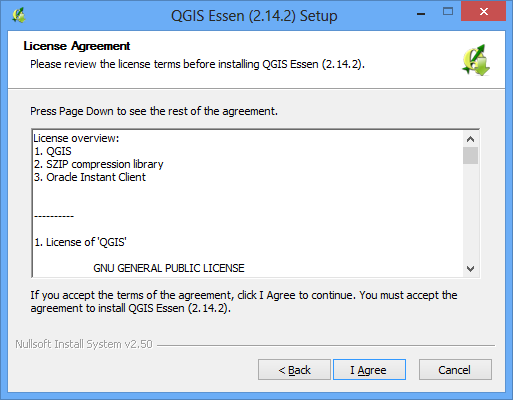
\includegraphics[width=0.9\textwidth]{./resources/install-win/003-license}
  \caption{Lisensi}
  \label{fig:agreement}
\end{figure}

\item Tentu saja pada jendela tersebut kita perlu menekan tombol \textit{I Agree} sehingga akan muncul tampilan seperti gambar \ref{fig:installlocation}

\begin{figure}[H]
  \centering
  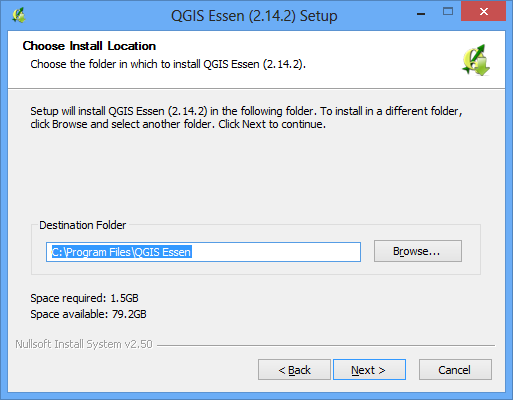
\includegraphics[width=0.9\textwidth]{./resources/install-win/004-install-location}
  \caption{Lokasi Instalasi}
  \label{fig:installlocation}
\end{figure}

\item Bila ingin mengubah lokasi instalasi dari QGIS, tekan tombol \textit{Browse} untuk memilih di \textit{folder} mana aplikasi akan ditempatkan, bila sudah selesai memilih lokasi instalasi, maka tekanlah tombol \textit{Next} sehingga akan muncul tampilan seperti pada gambar \ref{fig:qgiscomponent}

\begin{figure}[H]
  \centering
  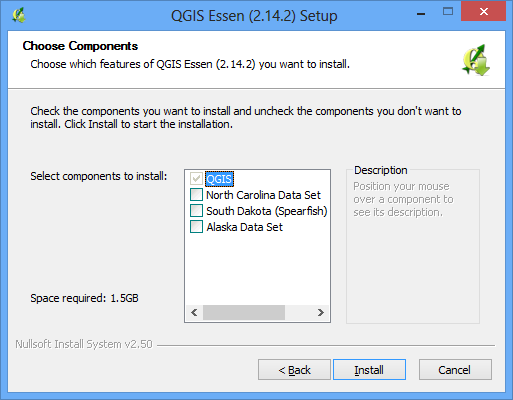
\includegraphics[width=0.9\textwidth]{./resources/install-win/005-component}
  \caption{Komponen QGIS Yang Akan Dipasang}
  \label{fig:qgiscomponent}
\end{figure}

\item Kita tidak akan menggunakan \textit{Data Set} yang disediakan karena hanya akan membuat proses instalasi berjalan lebih lama, cukup pilih komponen QGIS dan tekan tombol \textit{Install} sehingga muncul tampilan instalasi seperti gambar \ref{fig:prosesinstalasi}.

\begin{figure}[H]
  \centering
  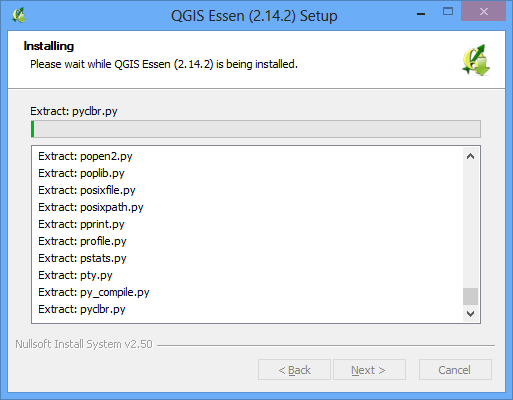
\includegraphics[width=0.9\textwidth]{./resources/install-win/006-installing}
  \caption{Proses Instalasi QGIS}
  \label{fig:prosesinstalasi}
\end{figure}

\item Tunggulah sampai proses instalasi sehingga muncul tampilan seperti pada gambar \ref{fig:finishinstalasi}, kemudian tekan tombol \textit{Finish} dan aplikasi QGIS siap digunakan.

\begin{figure}[H]
  \centering
  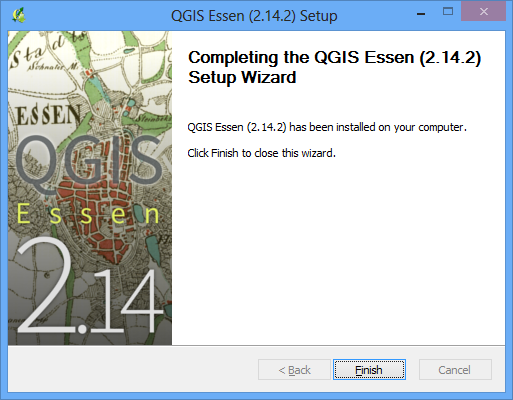
\includegraphics[width=0.9\textwidth]{./resources/install-win/007-finished}
  \caption{Instalasi QGIS Selesai}
  \label{fig:finishinstalasi}
\end{figure}

\end{enumerate}

\item Instalasi QGIS di lingkungan Sistem Operasi Linux (Debian/Ubuntu)

Instalasi QGIS di lingkungan sistem operasi linux berbeda-beda untuk setiap distro, pada pembahasan kali ini akan diuraikan dengan menggunakan distro dari keluarga Debian, yaitu Ubuntu.

\begin{enumerate}[1.]

\item Langkah pertamanya adalah mengubah isi dari \textit{file} \verb|/etc/apt/sources.list| agar Ubuntu dapat memahami dimana letak repositori QGIS berada. Isikan pada bagian paling bawah saja dengan baris kode berikut :

\begin{verbatim}
deb  http://qgis.org/debian trusty main
\end{verbatim}

atau 

\begin{verbatim}
deb http://qgis.org/ubuntugis trusty main
\end{verbatim}

Pada modul kali ini menggunakan repositori dari http://qgis.org/debian untuk distro Ubuntu versi 14.04 dengan nama alias \textit{trusty} untuk mendapatkan versi terbaru dari QGIS ini, yaitu versi 2.14 dengan nama alias \textit{essen}, sehingga dipilih opsi pertama. Sedangkan pada opsi kedua disajikan untuk distro Ubuntu versi 14.04 dengan versi QGIS berada pada 2.8 yang merupakan versi LTR (\textit{Long Term Release}).

\item Langkah selanjutnya adalah menjalankan perintah berikut pada konsol linux :

\begin{verbatim}
> sudo apt-get update
\end{verbatim}

Sehingga nanti daftar repositori \textit{software} akan terbaharui dan menambahkan sumber baru untuk melakukan instalasi QGIS.

\item Setelah repositori ter-\textit{update}, maka cukup menjalankan perintah berikut untuk instalasinya :

\begin{verbatim}
> sudo apt-get install qgis
\end{verbatim}

Tunggulah sampai selesai, dan aplikasi QGIS siap digunakan. 
\end{enumerate}

Jika aplikasi QGIS dijalankan, maka tampilannya akan terlihat seperti gambar \ref{fig:tampilan-awal-qgis}

\begin{figure}[H]
  \centering
  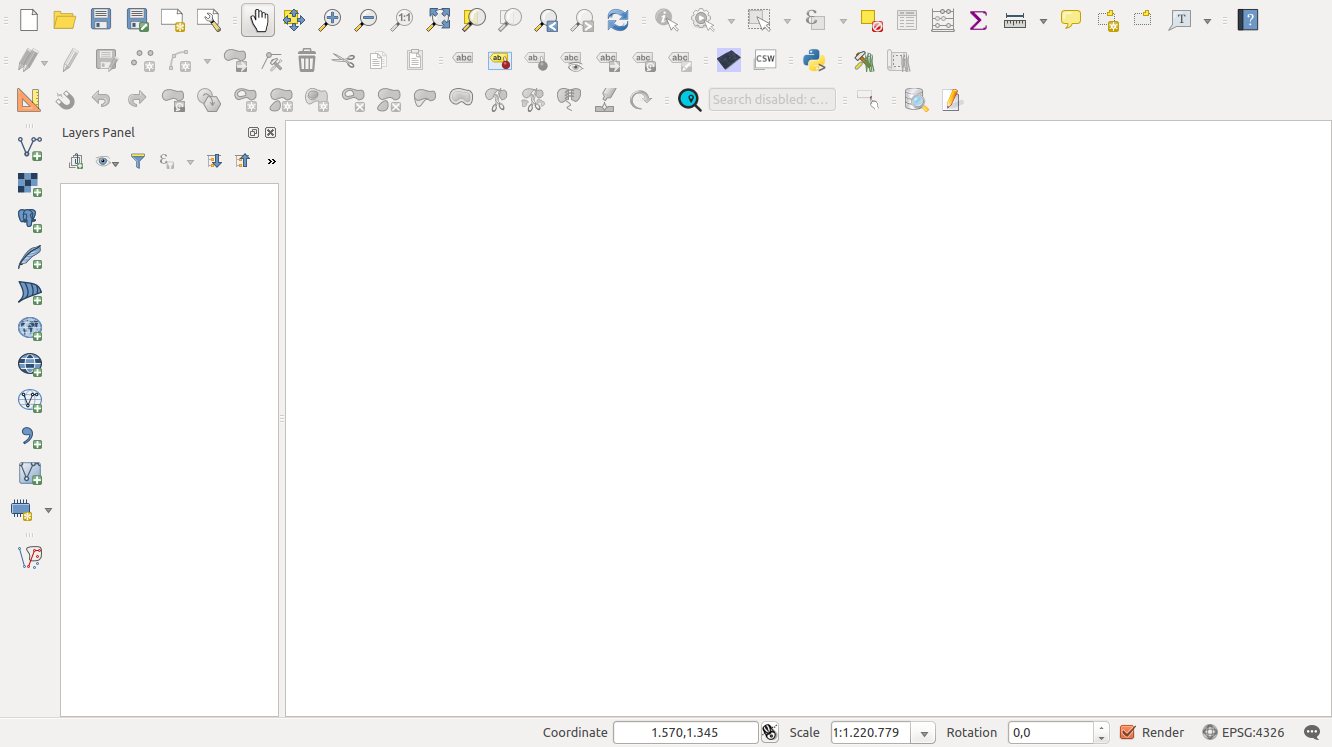
\includegraphics[width=1\textwidth]{./resources/003-jendela-awal-qgis}
  \caption{Jendela Awal QGIS}
  \label{fig:tampilan-awal-qgis}
\end{figure}

\end{enumerate}
